\chapter{Αποτελέσματα}
Παρακάτω θα παραθέσουμε τα αποτελέσματα των πειραμάτων μας. Προφανώς επειδή ο όγκος των πληροφοριών είναι αρκετά μεγάλος θα
παραλείψουμε τις περιπτώσεις που θεωρούμε πως δεν προσφέρουν κάποια χρήσιμη παρατήρηση η πληροφορία. \\~\\
Τα πειράματα μας χωρίζονται σε στατικά και μη-στατικά, όπου στην δεύτερη περίπτωση προσπαθήσαμε να προσομοιώσουμε την φυσική
κίνηση ενός ανθρώπου. Τα στατικά πειράματα χωρίζονται σε υποπεριπτώσεις που έχουν να κάνουν με το \te{line of sight} και τον
προσανατολισμό του \te{tag}. Επίσης, κάθε πείραμα περιλαμβάνει δεδομένα που δεν έχουν υποστεί καμία επεξεργασία ή φιλτράρισμα, καθώς θα εξετάσουμε την επίδραση
του φιλτραρίσματος παρακάτω. \\~\\
Τέλος, κάθε πείραμα περιλαμβάνει περίπου χίλιες μετρήσεις, δηλαδή περίπου δεκαεφτά μετρήσεις ανα δευτερόλεπτο. Στις περιπτώσεις που παραθέτουμε γραφικές
παραστάσεις, τα σημεία χρωματίζονται απο πράσινο σε μπλέ με την σειρά που υπολογίζονται.
\section{Στατικά Πειράματα με Απρόσκοπτο \te{Line Of Sight}}
Στα περισσότερα πειράματα πήραμε μετρήσεις σε τέσσερις θέσεις μέσα στο δωμάτιο και για κάθε τοποθεσία διεξάγαμε τρία ζευγάρια μετρήσεων
του ενός λεπτού. Κάθε ζευγάρι μετρήσεων χαρακτηρίζεται απο τον προσανατολισμό του \te{tag}, για παράδειγμα μια μέτρηση στην οποία το \te{tag} είναι
προσανατολισμένο διαγώνια ως προς τους άξονες \(x'x\) και \(y'y\) θα έχει σήμανση \te{\_diag}. Μια μέτρηση στην οποία η επιφάνεια του \te{tag} είναι
προσανατολισμένη ώς προς τον άξονα \(x'x\) θα έχει σήμανση \te{\_xx} και όμοια θα έχει σήμανση \te{\_yy} στην περίπτωση που η επιφάνεια του \te{tag}
είναι προσανατολισμένη ώς προς τον άξονα \(y'y\).
Τέλος, στο κάθε ζευγάρι μετρήσεων η πρώτη μέτρηση έχει σήμανση \te{\_A} ενώ η δεύτερη έχει σήμανση \te{\_B}.

Επίσης σημειώνουμε πως όλα τα στατικά πειράματα πραγματοποιήθηκαν στο δωμάτιο Α.
\subsection{Σύνοψη Αποτελεσμάτων}

Συνοψίζουμε τα αρχικά αποτελέσματα των δυο μεθόδων στους πίνακες 4.1 και 4.2. Επίσης, για ορισμένες περιπτώσεις επαναλάβαμε τα πειράματα μια διαφορετική μέρα, αυτά τα αποτελέσματα συνοψίζονται στους πίνακες 4.3 και 4.4.
\begin{table}[H]
    \centering
    \footnotesize
    \caption{Συνοπτικά Αποτελέσματα της μεθόδου Γεωμετρικού Βαρύκεντρου}
    \begin{tabular}{|l|l|l|l|l|}
    \hline
        & \te{BRC avg x} & \te{BRC avg y} & \te{BRC stdev x} & \te{BRC stdev y} ~ \\ \hline
        \te{278\_262\_diag\_A } & 205.56 & 258.7 & 12.2 & 5.8 \\ \hline
        \te{278\_262\_diag\_B }& 203.56 & 259.27 & 8 & 6 \\ \hline
        \te{278\_262\_xx\_A }& 320.54 & 330.44 & 223.9 & 141.6 \\ \hline
        \te{278\_262\_xx\_B }& 281.65 & 307.82 & 151.3 & 94.3 \\ \hline
        \te{278\_262\_yy\_A }& 244.46 & 253.84 & 5 & 8.1 \\ \hline
        \te{278\_262\_yy\_B }& 246.77 & 257.63 & 5.8 & 7.7 \\ \hline
        \te{283\_168\_diag\_A }& 210.41 & 158.07 & 3.5 & 3.5 \\ \hline
        \te{283\_168\_diag\_B }& 213.24 & 160.91 & 2.4 & 2.2 \\ \hline
        \te{283\_168\_xx\_A }& 215.38 & 145.6 & 3.4 & 6.8 \\ \hline
        \te{283\_168\_xx\_B }& 214.25 & 144.21 & 3.7 & 6.1 \\ \hline
        \te{283\_168\_yy\_A }& 222.32 & 150.61 & 12.5 & 7 \\ \hline
        \te{283\_168\_yy\_B }& 219.02 & 150.68 & 3 & 7.8 \\ \hline
        \te{400\_170\_diag\_A }& 360.69 & 151.02 & 0.7 & 2 \\ \hline
        \te{400\_170\_diag\_B }& 359.56 & 147.84 & 1 & 15.1 \\ \hline
        \te{400\_170\_xx\_A} & 364.05 & 122.47 & 2 & 7.8 \\ \hline
        \te{400\_170\_xx\_B }& 364 & 126.68 & 1.2 & 5.2 \\ \hline
        \te{400\_170\_yy\_A }& 401.08 & 170.98 & 1.7 & 3.6 \\ \hline
        \te{400\_170\_yy\_B }& 401.83 & 172.31 & 1.6 & 3.2 \\ \hline
        \te{504\_162\_diag\_A }& 490.57 & 188.97 & 4.6 & 8.5 \\ \hline
        \te{504\_162\_diag\_B }& 490.99 & 191.77 & 4.4 & 9.1 \\ \hline
        \te{504\_162\_xx\_A }& 475.71 & 155.74 & 2.8 & 7.8 \\ \hline
        \te{504\_162\_xx\_B }& 476.25 & 158.73 & 2.5 & 9.5 \\ \hline
        \te{504\_162\_yy\_A }& 539.36 & 328.9 & 21.2 & 34.4 \\ \hline
        \te{504\_162\_yy\_B }& 573.19 & 384.89 & 611.5 & 859.5 \\ \hline
    \end{tabular}
\end{table}

\begin{table}[H]
    \centering
    \footnotesize
    \caption{Συνοπτικά Αποτελέσματα της μεθόδου Ελάχιστων Τετραγώνων}
    \begin{tabular}{|l|l|l|l|l|}
    \hline
        & \te{LSQ avg x} & \te{LSQ avg y} & \te{LSQ stdev x} & \te{LSQ stdev y} ~ \\ \hline
        \te{278\_262\_diag\_A } & 254.13 & 268.34 & 5.5 & 3.5 \\ \hline
        \te{278\_262\_diag\_B  }& 254.34 & 269.22 & 4.5 & 3.6 \\ \hline
        \te{278\_262\_xx\_A } & 220.72 & 267.38 & 6.1 & 4.7 \\ \hline
        \te{278\_262\_xx\_B  }& 221.41 & 267.61 & 5.8 & 5.5 \\ \hline
        \te{278\_262\_yy\_A  }& 251.1 & 254.38 & 3.9 & 5.6 \\ \hline
        \te{278\_262\_yy\_B  }& 250.16 & 256.38 & 4.6 & 5.3 \\ \hline
        \te{283\_168\_diag\_A  }& 210.53 & 161.84 & 3.6 & 3.1 \\ \hline
        \te{283\_168\_diag\_B  }& 213 & 164.41 & 2.5 & 2.1 \\ \hline
        \te{283\_168\_xx\_A } & 217.53 & 148.27 & 3.7 & 4.5 \\ \hline
        \te{283\_168\_xx\_B  }& 217.02 & 148.27 & 3.9 & 3.9 \\ \hline
        \te{283\_168\_yy\_A  }& 225.2 & 157.32 & 11.9 & 4.9 \\ \hline
        \te{283\_168\_yy\_B  }& 222.38 & 157.91 & 2.2 & 5.3 \\ \hline
        \te{400\_170\_diag\_A  }& 360.09 & 151.47 & 0.8 & 2 \\ \hline
        \te{400\_170\_diag\_B } & 358.77 & 151.95 & 1.2 & 9.8 \\ \hline
        \te{400\_170\_xx\_A } & 366.19 & 123.39 & 2 & 7.6 \\ \hline
        \te{400\_170\_xx\_B } & 366.58 & 127.66 & 1.5 & 5.1 \\ \hline
        \te{400\_170\_yy\_A  }& 399.26 & 175.72 & 1.5 & 3.4 \\ \hline
        \te{400\_170\_yy\_B } & 399.99 & 177.05 & 1.4 & 2.9 \\ \hline
        \te{504\_162\_diag\_A  }& 483.25 & 177.75 & 3.5 & 6.2 \\ \hline
        \te{504\_162\_diag\_B  }& 482.49 & 179.61 & 3.3 & 6.4 \\ \hline
        \te{504\_162\_xx\_A } & 474.08 & 151.72 & 2.6 & 5.5 \\ \hline
        \te{504\_162\_xx\_B } & 474.52 & 154.51 & 2.4 & 6.7 \\ \hline
        \te{504\_162\_yy\_A } & 425.75 & 234.61 & 11.2 & 4.9 \\ \hline
        \te{504\_162\_yy\_B  }& 403.46 & 240.55 & 23.9 & 6.4 \\ \hline
    \end{tabular}
\end{table}

\begin{table}[H]
    \centering
    \footnotesize
    \caption{Αποτελέσματα δεύτερων μετρήσεων της μεθόδου Γεωμετρικού Βαρύκεντρου}
    \begin{tabular}{|l|l|l|l|l|}
    \hline
        & \te{BRC avg x} & \te{BRC avg y} & \te{BRC stdev x} & \te{BRC stdev y} ~ \\ \hline
        \te{292\_264\_diag\_A }& 233.4 & 273.34 & 6.7 & 11.3 \\ \hline
        \te{292\_264\_diag\_B }& 228.62 & 256.34 & 5.7 & 5.5 \\ \hline
        \te{281\_168\_diag\_A} & 206.14 & 136.09 & 5.6 & 3.9 \\ \hline
        \te{298\_167\_diag\_B} & 229.82 & 169.65 & 2.4 & 5 \\ \hline
        \te{400\_168\_diag\_A} & 360.92 & 178.63 & 1.9 & 13.2 \\ \hline
        \te{401\_166\_diag\_B} & 379.33 & 206.35 & 1.6 & 4.7 \\ \hline
        \te{405\_170\_yy\_A }  & 337.84 & 178.26 & 2.4 & 23.8 \\ \hline
        \te{405\_170\_yy\_B}   & 339.03 & 181.96 & 2.4 & 18.1 \\ \hline
        \te{410\_175\_xx\_A}   & 377.24 & 172.01 & 1.5 & 16.5 \\ \hline
        \te{410\_175\_xx\_B}   & 376.84 & 167.14 & 1.8 & 15.3 \\ \hline
        \te{519\_168\_diag\_A} & 483.79 & 191.09 & 2.1 & 6.4 \\ \hline
        \te{501\_160\_diag\_B} & 473.24 & 151.86 & 4.7 & 4 \\ \hline
        \te{504\_165\_yy\_A }  & 474.86 & 166.99 & 12.3 & 28.2 \\ \hline
        \te{504\_165\_yy\_B}  & 474.1 & 168.77 & 4.2 & 15.5 \\ \hline
    \end{tabular}
\end{table}

\begin{table}[H]
    \centering
    \footnotesize
    \caption{Αποτελέσματα δεύτερων μετρήσεων της μεθόδου Ελάχιστων Τετραγώνων}
    \begin{tabular}{|l|l|l|l|l|}
    \hline
        & \te{LSQ avg x} & \te{LSQ avg y} & \te{LSQ stdev x} & \te{LSQ stdev y} ~ \\ \hline
        \te{292\_264\_diag\_A }& 269.92 & 280.25 & 9.4 & 8.1 \\ \hline
        \te{292\_264\_diag\_B }& 264.11 & 268.82 & 3.9 & 3.9 \\ \hline
        \te{281\_168\_diag\_A} & 209.7 & 145.55 & 5.5 & 3.3 \\ \hline
        \te{298\_167\_diag\_B} & 230.2 & 168.46 & 2.4 & 3.7 \\ \hline
        \te{400\_168\_diag\_A} & 360.47 & 180.36 & 2.3 & 10.6 \\ \hline
        \te{401\_166\_diag\_B} & 378.52 & 205.21 & 1.8 & 4.6 \\ \hline
        \te{405\_170\_yy\_A }  & 340.86 & 188.57 & 2.5 & 8.6 \\ \hline
        \te{405\_170\_yy\_B}   & 341.6 & 186.55 & 2.4 & 4.3 \\ \hline
        \te{410\_175\_xx\_A}   & 378.96 & 170.35 & 3.4 & 15.2 \\ \hline
        \te{410\_175\_xx\_B}   & 377.33 & 166.25 & 1.9 & 14.8 \\ \hline
        \te{519\_168\_diag\_A} & 482.45 & 189.33 & 2.4 & 4.8 \\ \hline
        \te{501\_160\_diag\_B} & 469.35 & 145.47 & 5.2 & 3.1 \\ \hline
        \te{504\_165\_yy\_A }  & 467.91 & 160.04 & 8.3 & 18.7 \\ \hline
        \te{504\_165\_yy\_B}  & 470.72 & 162.11 & 3.8 & 11.3 \\ \hline
    \end{tabular}
\end{table}

\subsection{Αξιοσημείωτες Περιπτώσεις}
Στην συνέχεια θα εξετάσουμε απο κοντά ορισμένες περιπτώσεις που θεωρούμε πως αξίζουν ιδιαίτερη προσοχή. \\~\\
\subsubsection{\te{278\_262\_xx}}
Αρχικά ξεκινάμε με την περίπτωση γεωμετρικού βαρυκέντρου \te{278\_262\_xx} του πίνακα 4.1. Και στις δυο περιπτώσεις Α και Β βλέπουμε πως πρώτον υπάρχει
έντονη απόκλιση μεταξύ των πραγματικών και των υπολογισμένων συντεταγμέων, \((278, 262)\) με \((320, 330)\) και \((281, 307)\). Υπάρχει όμως και μια
πολύ μεγάλη τυπική απόκλιση η οποία σε γενικές γραμμές δεν παρατηρείται σε άλλα πειράματα. Παρολαυτά, στην περίπτωση των ελαχίστων τετραγώνων τόσο το
σφάλμα στις συντεταγμένες όσο και η τυπική απόκλιση των τιμών είναι σε πολύ πιο λογικά πλαίσια. \\~\\

\begin{figure}[h]
\centering
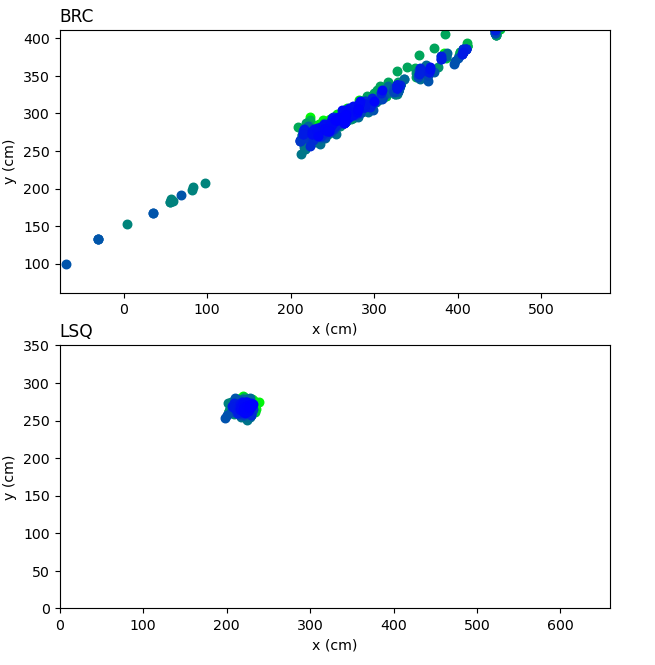
\includegraphics[width=7cm]{pictures/results_a.png}
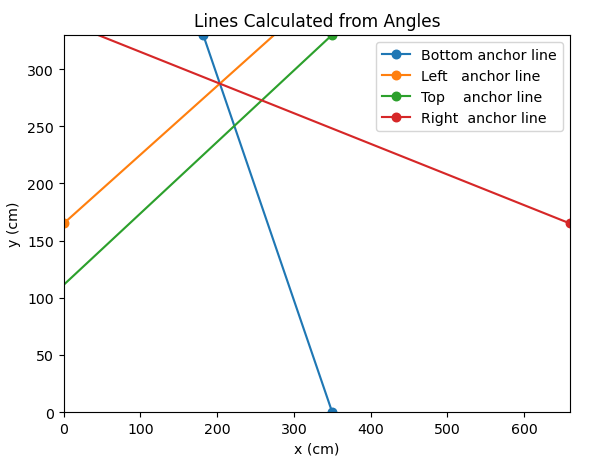
\includegraphics[width=7cm]{pictures/results_a1.png}
\caption{Γραφική παράσταση του πειράματος \te{278\_262\_xx\_A}}
\end{figure}
Όπως φαίνεται και γραφικά στο σχήμα 4.1\te{a} η μέθοδος του βαρύκεντρου αποτυγχάνει έντονα σε αυτήν την συγκεκριμένη περίπτωση. Στην πραγματικότητα αυτό δεν
είναι τυχαίο αλλά οφείλεται σε μια βασική αδυναμία της συγκεκριμένης μεθόδου. Στο σχήμα 4.1\te{b} θα παρατηρήσουμε της ευθείες που δημιουργούνται απο μια τυχαία τετράδα γωνιών του πειράματος αυτού. Βλέπουμε πως δυο ευθείες απο τις οποίες θέλουμε να υπολογίσουμε το σημείο τομής είναι σχεδόν παράλληλες.
Έτσι λοιπόν τα σημεία που παράγονται απο αυτόν τον υπολογισμό είναι προβληματικά.


Στο σχήμα 4.2 θα δούμε τις χρονοσειρές που σχηματίζονται απο τις μετρήσεις των γωνιών. Εκεί παρατηρούμε πως το \te{left anchor} είναι εμφανώς πιο θορυβώδες
απο τα υπόλοιπα. Αυτό είναι ενα φαινόμενο που όπως θα δούμε είναι παρών σε πολλές μετρήσεις.

\begin{figure}[h]
\centering
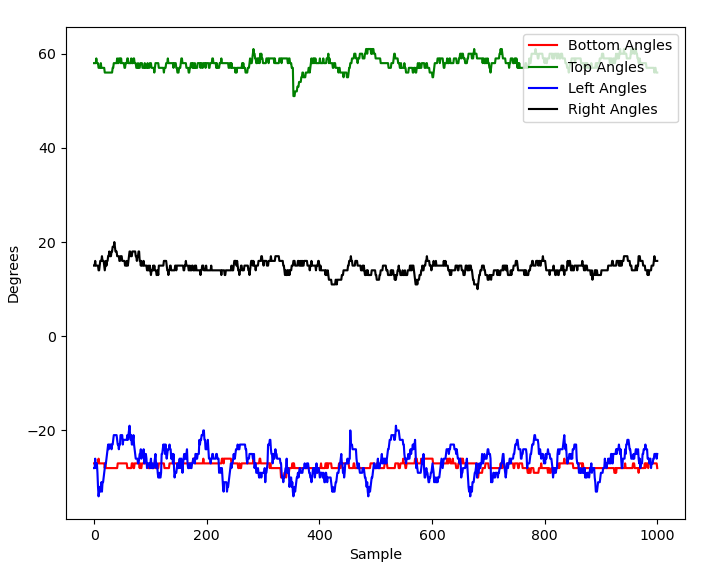
\includegraphics[width=8cm]{pictures/results_a2.png}
\caption{Χρονοσειρές γωνιών για το πείραμα \te{278\_262\_xx\_A}}
\end{figure}

\subsubsection{\te{504\_162\_yy\_B}}
Η επόμενη περίπτωση που θα εξετάσουμε είναι το πείραμα \te{504\_162\_yy\_B} του πίνακα 4.1. Βλέπουμε πως οι τυπικές αποκλίσεις των συντεταγμένων είναι πολύ
υψηλές, 611 για το \(x\) και 859 για το \(y\). Στο σχήμα 4.3\te{a} θα δούμε την γραφική παράσταση του πειράματος και στο 4.3\te{b} θα δούμε τις ευθείες που σχηματίζονται απο μια τυχαία τετράδα γωνιών. Τέλος στο σχήμα 4.4 θα δούμε την χρονοσειρά των γωνιών του πειράματος.
\begin{figure}[h]
\centering
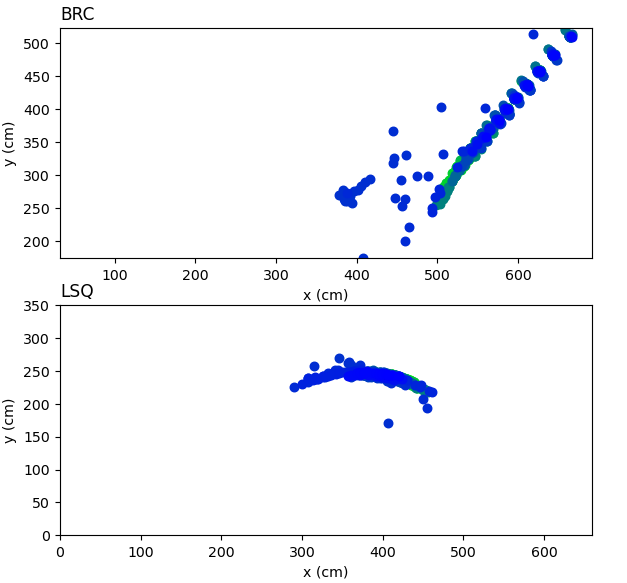
\includegraphics[width=7cm]{pictures/results_b.png}
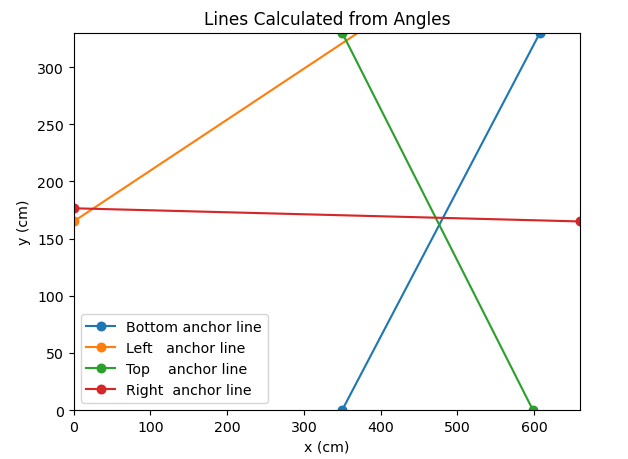
\includegraphics[width=7cm]{pictures/results_b1.png}
\caption{Γραφική παράσταση του πειράματος \te{504\_162\_yy\_B}}
\end{figure}

\begin{figure}[h]
\centering
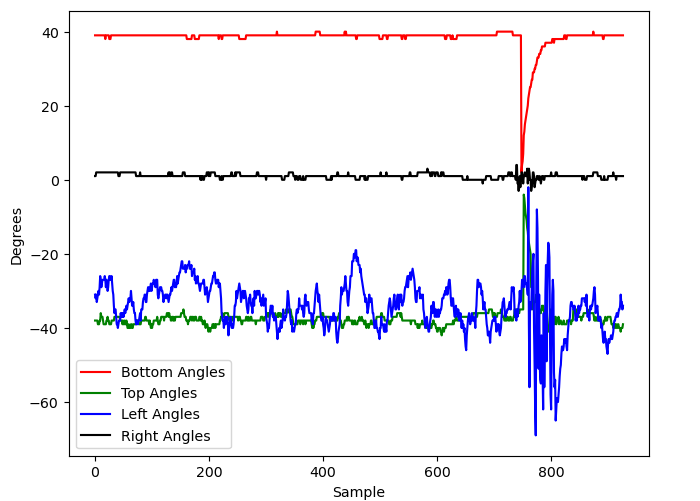
\includegraphics[width=8cm]{pictures/results_b2.png}
\caption{Χρονοσειρές γωνιών για το πείραμα \te{504\_162\_yy\_B}}
\end{figure}

Παρατηρούμε για μια ακόμα φορά πως το \te{left anchor} είναι θορυβώδες και για αυτόν τον λόγο η μέθοδος του βαρύκεντρου αποτυγχάνει. Για να αποδείξουμε
πως πραγματικά εφθύνετε το αυτό το \te{anchor} για το πρόβλημα, τροποποιήσαμε τον αλγόριθμο ώστε μήν το χρησιμοποιεί στους υπολογισμούς του. Στο σχήμα 4.5
θα δούμε τα αποτελέσματα στην περίπτωση που οι αλγόριθμοι βαρύκεντρου και ελαχίστων τετραγώνων δεν χρησιμοποιούν το \te{left anchor} στους υπολογισμούς τους.

Επίσης, στο σχήμα 4.4 βλέπουμε πως υπάρχει ένα \te{spike} στις τιμές των γωνιών όλων των κεραιών την ίδια χρονική στιγμή. Αυτό το αποδίδουμε σε κάποια
ηλεκτρομαγνητική παρεμβολή.
\begin{figure}[H]
\centering
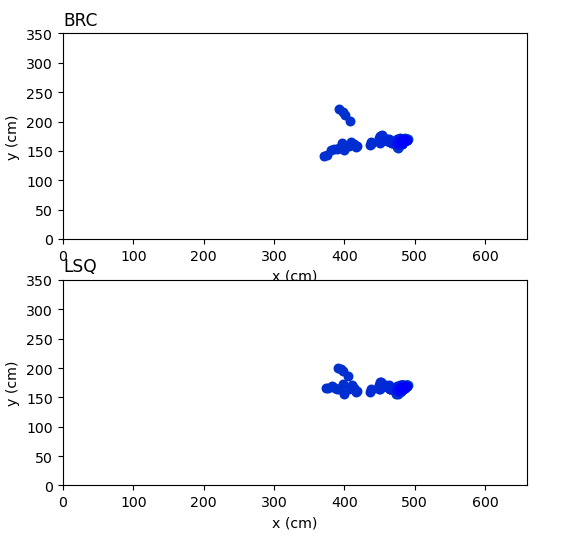
\includegraphics[width=8cm]{pictures/results_b3.png}
\caption{Γραφική παράσταση του \te{504\_162\_yy\_B} όταν δεν χρησιμοποιείται το \te{left anchor}}
\end{figure}

Είναι φανερό πως στην περίπτωση του σχήματος 4.5 τα αποτελέσματα είναι καλύτερα και οι μέθοδοι συγκλίνουν πολύ περισσότερο στα αποτελέσματα τους. Με αυτά τα
δυο παραδείγματα βλέπουμε γρήγορα πως η μέθοδος του βαρύκεντρου έχει αδυναμίες που η μέθοδος των ελάχιστων τετραγώνων δεν έχει.

Έχει ενδιαφέρον να δούμε το ίδιο πείραμα το οποίο όμως διεξήχθει μια άλλη μέρα. Δηλαδή να δούμε τον πίνακα 4.3-4.4.
Βλέπουμε πως αυτήν την φορά η μέση τιμή είναι \((470, 162)\). Στο σχήμα 4.6 βλέπουμε την γραφική παράσταση του πειράματος
\begin{figure}[H]
\centering
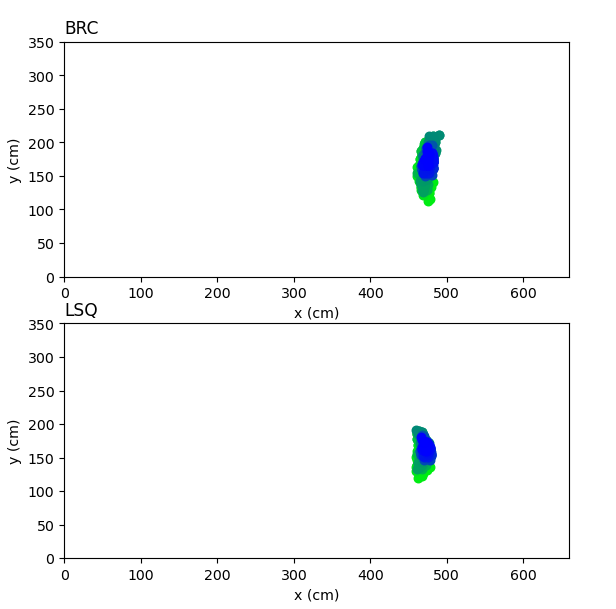
\includegraphics[width=7cm]{pictures/results_b4.png}
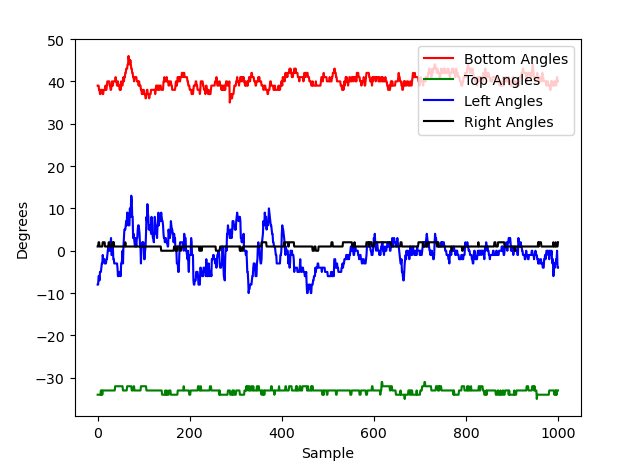
\includegraphics[width=7cm]{pictures/results_b5.png}
\caption{Γραφική παράσταση και χρονοσειρά γωνιών του \te{504\_165\_yy\_B} που διεξήχθει σε άλλη μέρα}
\end{figure}

Το συγκεκριμένο πείραμα μας δίχνει πως και οι δυο μέθοδοι είναι αρκετά ευαίσθητες σε τυχαίες μεταβολές του περιβάλλοντος, μεταβολές οι οποίες σε γενικές γραμμές δεν
μπορούν να προβλεφθούν.

\subsubsection{\te{400\_170\_yy\_A}}
Στην συνέχεια θα εξετάσουμε μια περίπτωση που τα αποτελέσματα είναι ιδιαίτερα καλά αντί για ιδιαίτερα άσχημα. Στο πείραμα \te{400\_170\_yy\_A} και στην περίπτωση
του βαρύκεντρου και των ελάχιστων τετραγώνων βλέπουμε ιδιαίτερα καλά αποτελέσματα τόσο σε τιμή όσο και στην τυπική απόκλιση, όπως φαίνεται στο σχήμα 4.7
\begin{figure}[H]
\centering
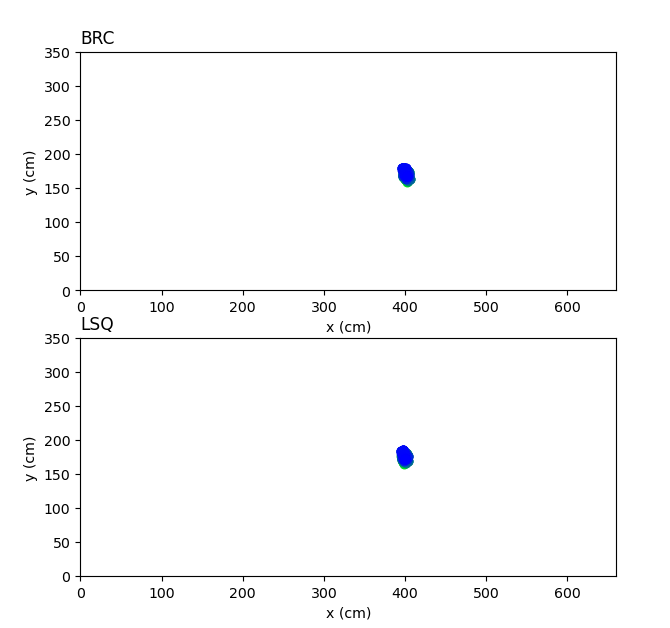
\includegraphics[width=8cm]{pictures/results_c.png}
\caption{Γραφική παράσταση για το πείραμα \te{400\_170\_yy\_A}}
\end{figure}

Η μέση τιμή για την μέθοδο του βαρύκεντρου είναι \((401, 170)\) ενώ για την περίπτωση των ελάχιστων τετραγώνων \((399, 175)\), και οι δύο περιπτώσεις είναι σχεδόν τέλειες. Στο σχήμα 4.8 βλέπουμε τις χρονοσειρές των γωνιών για αυτό το πείραμα, μπορούμε να δούμε πως δεν υπάρχει κάποιος έντονος θόρυβος σε κανένα \te{anchor}.
Το γεγονός πως η μέτρηση είναι σχεδόν στο κέντρο του δωματίου αλλά και το γεγονός πως οι μετρήσεις των γωνιών ήταν αρκετά καλές
και αθόρυβες συμβάλουν στο πολύ καλό
τελικό αποτέλεσμα.
\begin{figure}[H]
\centering
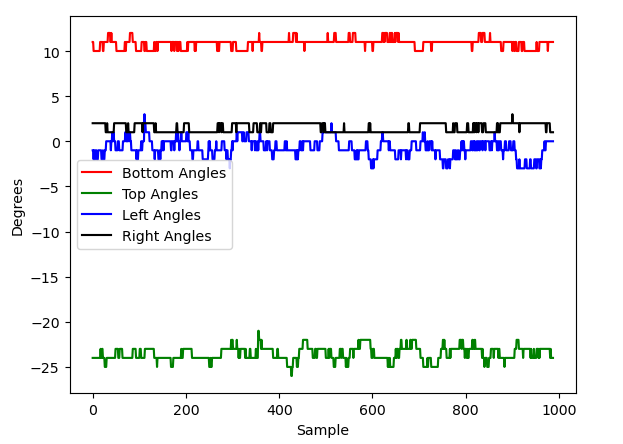
\includegraphics[width=8cm]{pictures/results_c1.png}
\caption{Χρονοσειρές γωνιών για το πείραμα \te{400\_170\_yy\_A}}
\end{figure}

\subsection{Επίδραση του Προσανατολισμού του \te{tag}}
Παρακάτω θα εξετάσουμε την επίδραση του προσανατολισμόυ του \te{tag} με ορισμένα παραδείγματα.
Αρχικά παρουσιάζουμε μια σύνοψη στον πίνακα 4.5. Απο εδώ και πέρα είναι προφανές πως η μέθοδος των ελάχιστων τετραγώνων είναι η πιό σταθερή, για αυτόν τον λόγο και εμείς θα αναλύσουμε μόνο τα αποτελέσματα που παράχθηκαν απο αυτήν.

Έπειτα, θεωρώντας πως η τυπική απόκλιση είναι μια καλή μετρική για την μη-κανονικότητα της χρονοσειράς των γωνιών, στο σχήμα 4.9\te{a} ώς 4.9\te{d}
θα παρουσιάσουμε τις τυπικές αποκλίσεις για τις διάφορες περιπτώσεις.
\begin{table}[H]
    \centering
    \footnotesize
    \caption{Σύγκριση αποτελεσμάτων προσανατολισμού για την μέθοδο ελάχιστων τετραγώνων}
    \begin{tabular}{|l|l|l|l|l|}
    \hline
        & \te{xx} & \te{yy} & \te{diag} & \te{outlier} \\ \hline
        \te{278\_262\_A} & (220, 267) & (251, 254) & (254, 268) & \te{soft xx} \\ \hline
        \te{283\_168\_A} & (217, 148) & (225, 157) & (210, 161) & - \\ \hline
        \te{400\_170\_A} & (366, 123) & (399, 175) & (360, 151) & \te{yy} \\ \hline
        \te{504\_162\_A} & (474, 151) & (425, 234) & (483, 177) & \te{yy} \\ \hline
    \end{tabular}
\end{table}

\begin{figure}[H]
\centering
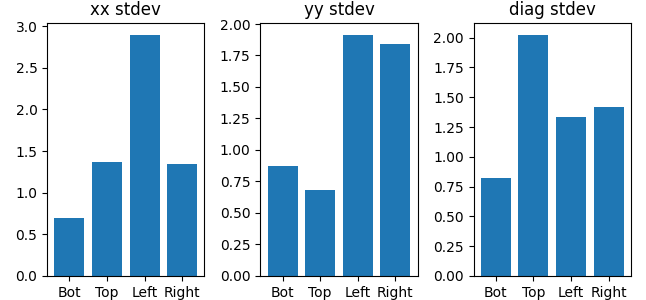
\includegraphics[width=7cm]{pictures/stdevs_278_262_A.png}
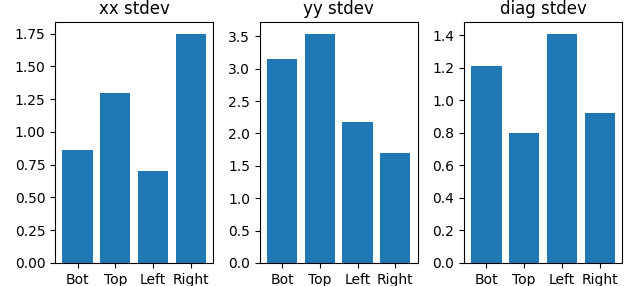
\includegraphics[width=7cm]{pictures/stdevs_283_168_A.png}
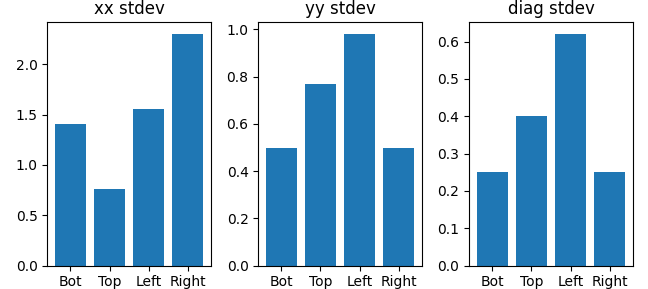
\includegraphics[width=7cm]{pictures/stdevs_400_170_A.png}
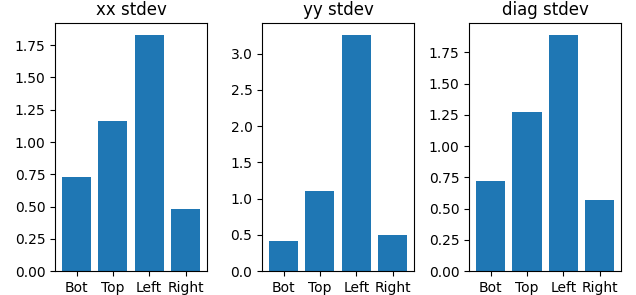
\includegraphics[width=7cm]{pictures/stdevs_504_162_A.png}
\caption{Τυπικές Αποκλίσεις για τα πειράματα \te{278\_262\_A (a)}, \te{283\_168\_A (b)}, \te{400\_170\_A (c)} και \te{504\_162\_A (d)}}
\end{figure}

Βλέπουμε πως στο σχήμα \te{4.9a} η χειρότερη τιμή βρίσκεται κατα τον προσανατολισμό \te{xx}, στο σχήμα \te{4.9b} η χειρότερη τιμή βρίσκεται κατα τον προσανατολισμό \te{yy}, στο σχήμα \te{4.9c} η χειρότερη τιμή βρίσκεται κατα τον προσανατολισμό \te{xx} και στο σχήμα \te{4.9d} η χειρότερη τιμή βρίσκεται κατα τον προσανατολισμό \te{yy}.

Προφανώς ο θόρυβος που εισάγεται στα σήματα των γωνιών δεν ευθύνεται μόνο στον προσανατολισμό του \te{tag} αλλά και σε διάφορα
απρόβλεπτα ηλεκτρομαγντικά φαινόμενα, παρολαυτά μπορούμε να συμπεράνουμε πως ο διαγώνιος προσανατολισμός έχει σε γενικές γραμμές την
μεγαλύτερη κανονικότητα.

Τώρα θα εξετάσουμε μια περίπτωση στην οποία ο διαγώνιος προσανατολισμός είναι χειρότερος. \\

\subsubsection{\te{400\_170\_diag\_B}}
Το πείραμα \te{400\_170\_diag\_B} είναι στην ίδια τοποθεσία με το \te{400\_170\_yy\_A} αλλά το \te{tag} βρίσκεται σε διαγώνιο
προσανατολισμό.
Αρχικά απο τους πίνακες 4.1 και 4.2 βλέπουμε πως οι μέσες τιμές που υπολογίζονται είναι \((359, 147)\) και \((358, 151)\) για την μέθοδο
του βαρύκεντρου και
των ελάχιστων τετραγώνων αντίστοιχα. Το ενδιαφέρον εδώ φαίνεται στο σχήμα 4.9, όπου βλέπουμε την χρονοσειρά των γωνιών.
\begin{figure}[H]
\centering
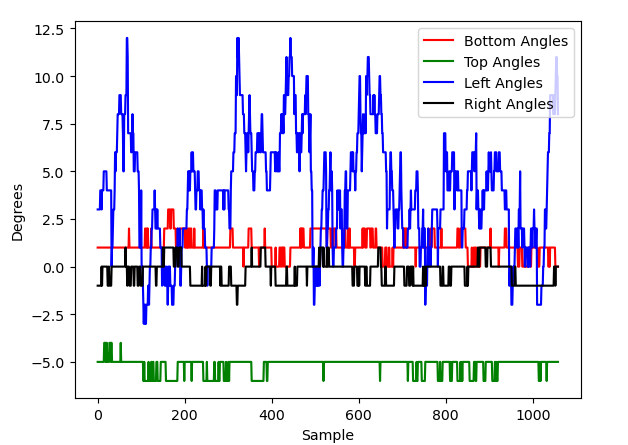
\includegraphics[width=8cm]{pictures/results_d1.png}
\caption{Χρονοσειρές γωνιών για το πείραμα \te{400\_170\_diag\_B}}
\end{figure}
Στο σχήμα 4.10 εμφανίζεται μια έντονη ταλάντωση στο \te{left anchor} που όμως δεν είναι προφανές αν ευθύνεται στον προσανατιλισμό,
στο σχήμα 4.11 βλέπουμε
το αποτέλεσμα αυτής της ταλάντωσης στα τελικά αποτελέσματα. Η ταλάντωση της τιμής της γωνίας εμφανίζεται σαν μια αντίστοιχη ταλάντωση
στις συντεταγμένες που υπολογίζονται.
\begin{figure}[H]
\centering
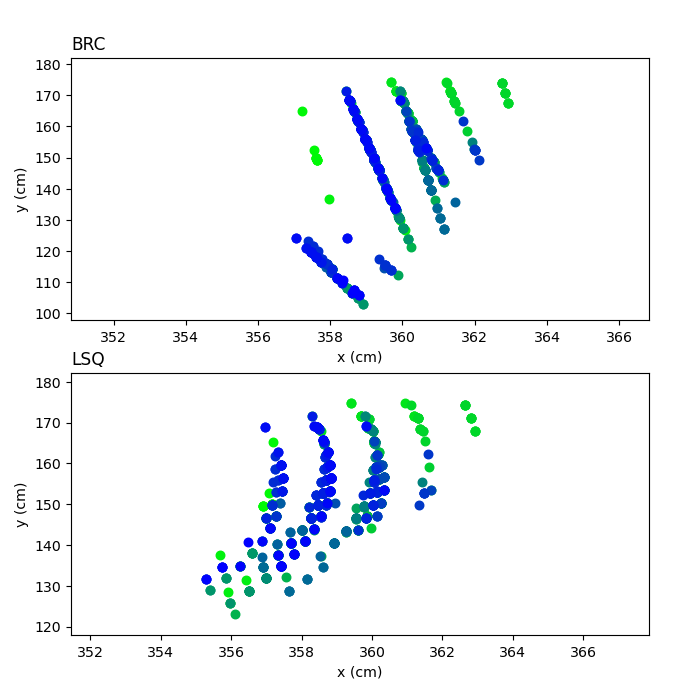
\includegraphics[width=8cm]{pictures/results_d.png}
\caption{Εστιασμένη γραφική παράσταση για το πείραμα \te{400\_170\_diag\_B}}
\end{figure}

\subsection{Επίδραση Θορυβώδους \te{Anchor}}
Όπως έχει γίνει εμφανές απο τα προηγούμενα παραδείγματα υπάρχουν πολλές περιπτώσεις που κάποιο \te{anchor}, συνήθως το \te{left anchor},
είναι θορυβώδες. Θα χρησιμοποιήσουμε μερικά παραδείγματα για να δείξουμε πως σε αυτές τις περιπτώσεις το να εξαιρούμε αυτό το \te{anchor}
απο τους υπολογισμούς μας, οδηγεί σε καλύτερα αποτελέσματα. Οι αλγόριθμοι τροποποιήθηκαν αντίστοιχα για αυτόν τον σκοπό. \\

\subsubsection{\te{400\_170\_diag\_B}}
Ξαναεξετάζουμε το πείραμα \te{400\_170\_diag\_B}.
\begin{figure}[H]
\centering
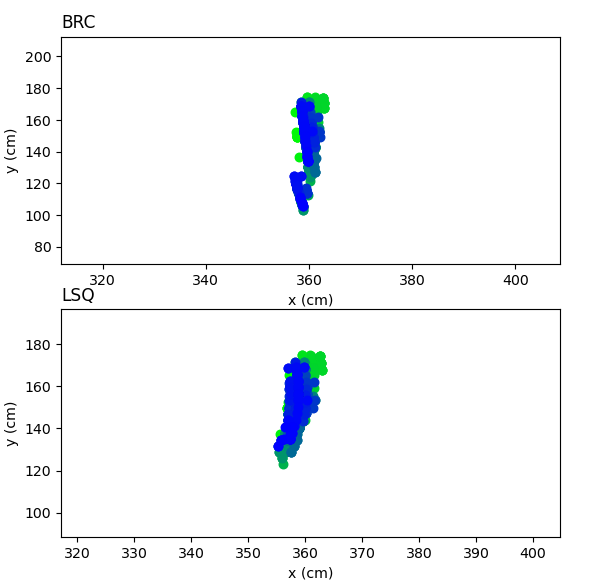
\includegraphics[width=7cm]{pictures/results_e1.png}
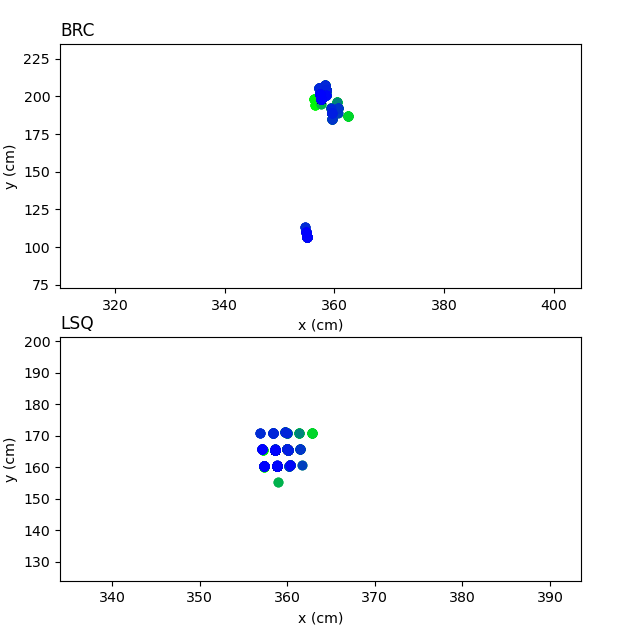
\includegraphics[width=7cm]{pictures/results_e.png}
\caption{Εστιασμένη γραφική παράσταση για το πείραμα \te{400\_170\_diag\_B} με το \te{left anchor (a)} και χωρίς αυτό (\te{b})}
\end{figure}

Στο σχήμα 4.12 φαίνεται η διαφορά στα αποτελέσματα με το \te{left anchor} και χωρίς αυτό. Έχοντας υπόψη μόνο την μέθοδο ελάχιστων τετραγώνων,
η μέση τιμή των σημείων στην περίπτωση \te{a} είναι \((358, 151)\) ενώ στην περίπτωση \te{b} είναι \((359, 164)\), επίσης οι τυπικές αποκλίσεις για τις συντεταγμένες
στην περίπτωση \te{a} είναι \(1.2, 9.8\) ενώ στην περίπτωση \te{b} είναι \(1, 3.2\).

Βλέπουμε πως οι μέσες τιμές είναι πιο κοντά στις πραγματικές συντεταγμένες, και επίσης πως οι τυπικές αποκλίσεις (ειδικά για τη συντεταγμένη \(y\)) είναι πολύ
πιο χαμηλές στην περίπτωση \te{b}.

Επίσης στο σχήμα 4.13 φαίνεται ακριβώς για ποιόν λόγο η ταλάντωση του \te{left anchor} προκαλεί τις διάσπαρτες συντεταγμένες \(y\)
\begin{figure}[H]
\centering
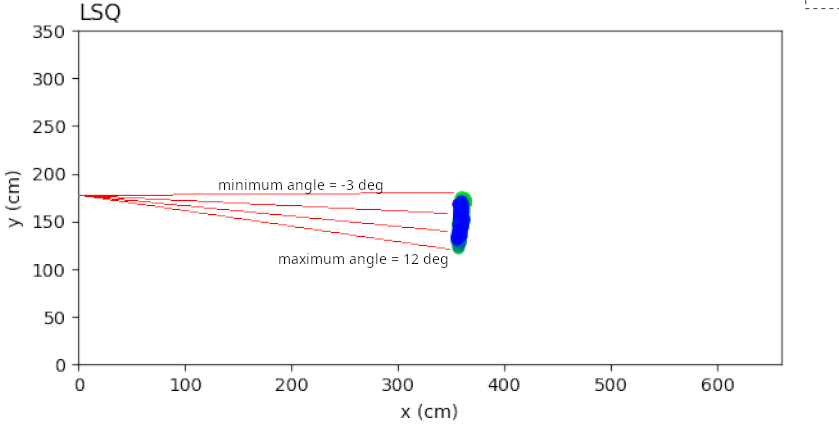
\includegraphics[width=10cm]{pictures/results_e2.png}
\caption{Γραφική παράσταση της ταλάντωσης του \te{left anchor}}
\end{figure}

\subsubsection{\te{504\_162\_yy\_A}}
Το δεύτερο παράδειγμα που θα δείξουμε είναι το πείραμα \te{504\_162\_yy\_A}. Αρχικά στο σχήμα 4.14 βλέπουμε τον θόρυβο του \te{left anchor}
και στο σχήμα 4.15 βλέπουμε την γραφική του παράσταση με το \te{left anchor (a)} και χωρίς αυτό \te{(b)}.
\begin{figure}[H]
\centering
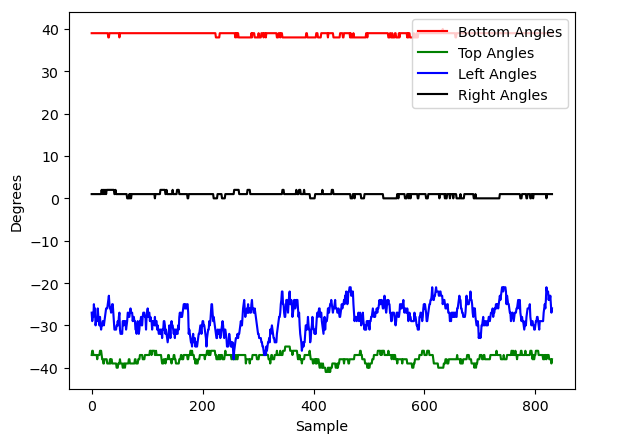
\includegraphics[width=8cm]{pictures/results_f.png}
\caption{Χρονοσειρές γωνιών για το πείραμα \te{504\_162\_yy\_A}}
\end{figure}

\begin{figure}[H]
\centering
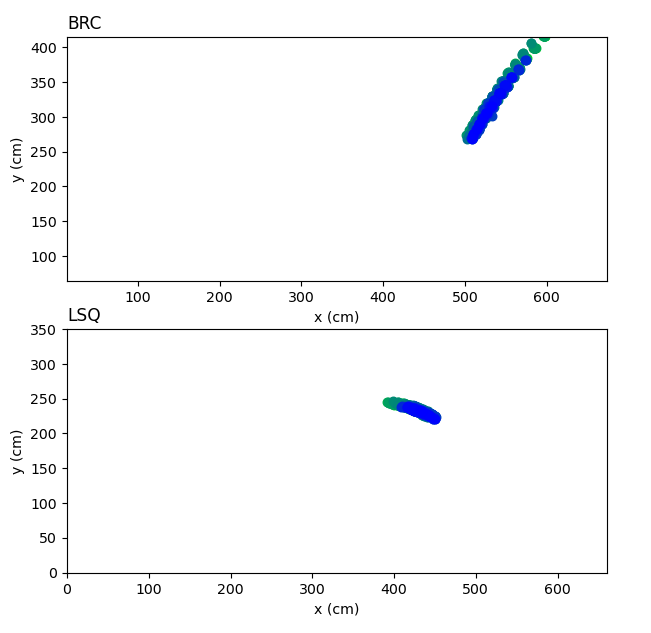
\includegraphics[width=7cm]{pictures/results_f1.png}
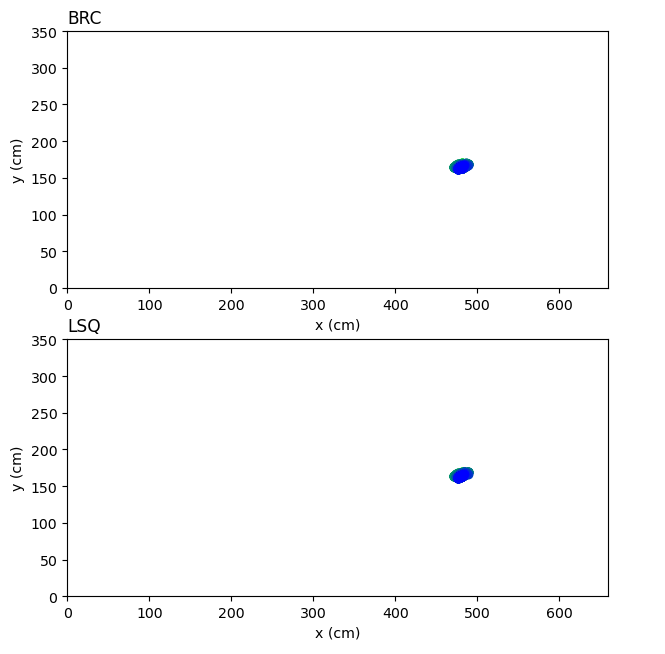
\includegraphics[width=7cm]{pictures/results_f2.png}
\caption{Γραφική παράσταση για το πείραμα \te{504\_162\_yy\_A} με το \te{left anchor (a)} και χωρίς αυτό (\te{b})}
\end{figure}

Σε αυτό το πείραμα οι μέσες τιμές της μεθόδος ελάχιστων τετραγώνων με το \te{left anchor} είναι \((425, 234)\) ενώ οι τυπικές αποκλίσεις είναι \(11.2, 4.9\).
Αντίθετα στην περίπτωση χωρίς το \te{left anchor} είναι \((479, 1165)\) και \(2.8, 1.8\). Είναι προφανές πως η εξαίρεση του θορυβώδους \te{anchor} βελτιώνει και
τις μέσες τιμές όσο και τις αποκλίσεις.

\section{Στατικά Πειράματα με Ανθρώπινο Εμπόδιο}
Εκτός απο την πλειονότητα των πειραμάτων με απρόσκοπτο \te{line of sight}, πηραμε και μερικά πειράματα στα οποία το ανθρώπινο σώμα δημιουργεί κάποιο εμπόδιο στο \te{line of sight}.
\subsection{Σύνοψη Αποτελεσμάτων}
Τα αποτελέσματα για τα τρία πειράματα φαίνονται στον πίνακα 4.6
\begin{table}[H]
    \centering
    \footnotesize
    \caption{Σύνοψη αποτελεσμάτων πειραμάτων με ανθρώπινο εμπόδειο}
    \begin{tabular}{|l|l|l|l|l|}
    \hline
        & \te{LSQ avg x} & \te{LSQ avg y} &\te{LSQ stdev x} &\te{LSQ stdev y} \\ \hline
        \te{400\_170\_diag\_H\_A} & 358 & 149 & 3.6 & 16.6 \\ \hline
        \te{400\_170\_diag\_H\_B} & 358 & 178 & 1.9 & 22.5 \\ \hline
        \te{400\_170\_diag\_H\_C} & 355 & 169 & 3.6 & 8    \\ \hline
    \end{tabular}
\end{table}

\subsection{Αναλυτικά Αποτελέσματα}
\subsubsection{\te{400\_170\_diag\_H\_A}}
Στο πρώτο πείραμα με ανθρώπινο εμπόδιο, ένας άνθρωπος διέγραφε κυκλικές κινήσεις γύρω απο το \te{tag}, σε ρυθμό περπατήματος.
Στο σχήμα 4.16 βλέπουμε την χρονοσειρά των γωνιών του πειράματος.
\begin{figure}[H]
\centering
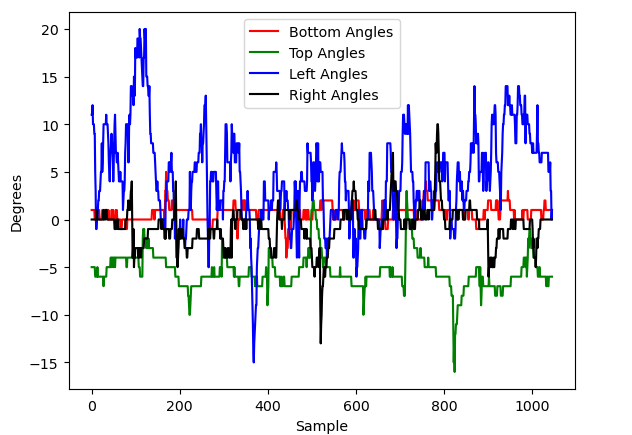
\includegraphics[width=8cm]{pictures/results_g.png}
\caption{Χρονοσειρές γωνιών για το πείραμα \te{400\_170\_diag\_H\_A}}
\end{figure}

Στο σχήμα 4.17(\te{a}) βλέπουμε την γραφική παράσταση του ίδιου πειράματος και στο 4.17\te{b} βλέπουμε τα αποτελέσματα αν δοκιμάσουμε να βγάλουμε το \te{left anchor}
απο τους υπολογισμούς μας, όπως πριν.
\begin{figure}[H]
\centering
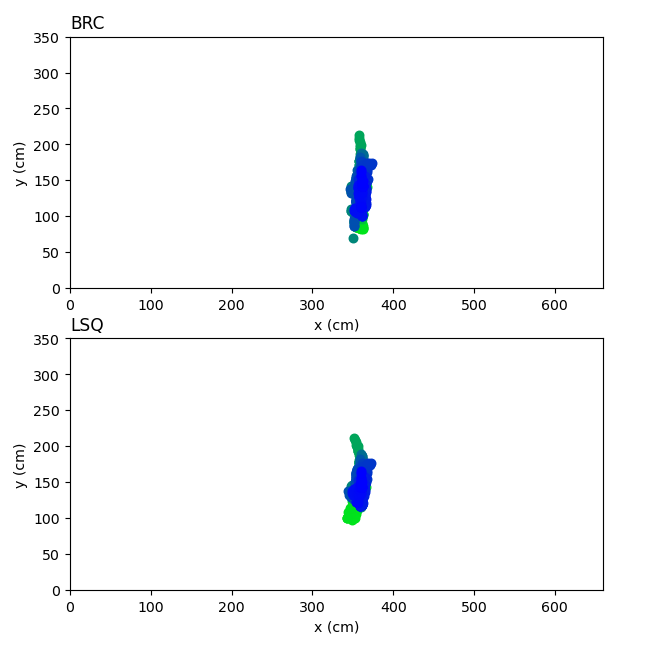
\includegraphics[width=7cm]{pictures/results_g1.png}
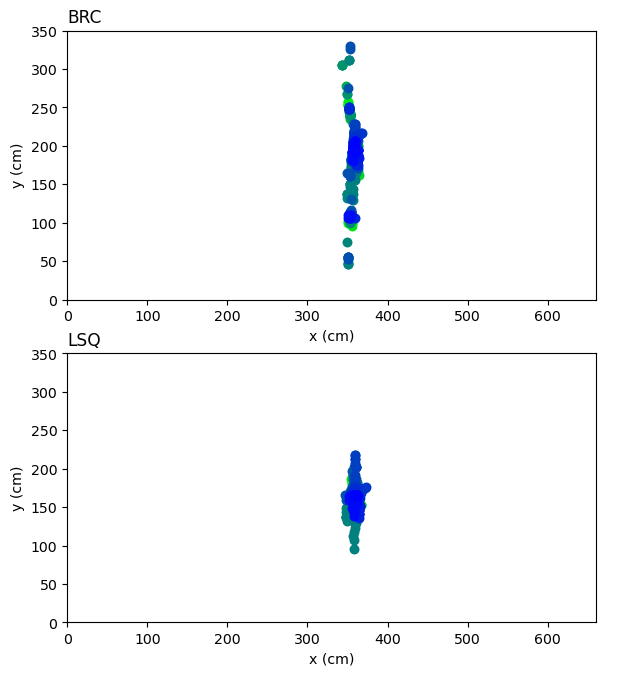
\includegraphics[width=7cm]{pictures/results_g2.png}
\caption{Γραφική παράσταση για το πείραμα \te{400\_170\_diag\_H\_A} με \te{left anchor (a)} και χωρίς αυτό \te{(b)}}
\end{figure}

Βλέπουμε πως αρχικά, η παρέμβαση του ανθρώπινου σώματος δημιουργεί έντονο θόρυβο σε όλα τα \te{anchor} και όχι μόνο στο \te{left anchor}, συγκεκριμένα οι τυπικές αποκλίσεις
γωνιών για τα τέσσερα \te{anchors} είναι \(0.82, 1.85, 4.87, 2.04\) με σειρά \te{bottom, top, left, right}. Έπειτα βλέπουμε πως σε αυτήν την περίπτωση, η εξαίρεση του
\te{left anchor} δεν βελτιώνει αισθητά τα αποτελέσματα καθώς όλα τα \te{anchors} είναι θορυβώδη.

\subsubsection{\te{400\_170\_diag\_H\_B}}
Στο πείραμα \te{400\_170\_diag\_H\_B} ένας άνθρωπος κάλυπτε με τα χέρια του το \te{tag} απτήν δεξιά πλευρά για τα πρώτα τριάντα δευτερόλεπτα
του πειράματος και έπειτα απτην αριστερή πλευρά για τα επόμενα 30 δευτερόλεπτα.
Στο σχήμα 4.18 βλέπουμε τις χρονοσειρές γωνιών για το πειράματα ενώ στο 4.19 βλέπουμε την γραφική παράσταση του.
\begin{figure}[H]
\centering
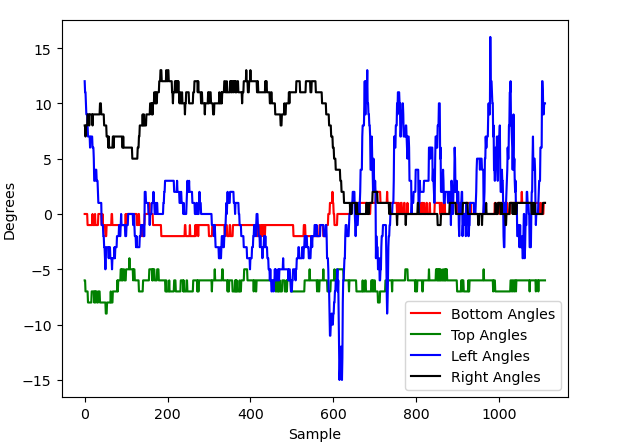
\includegraphics[width=8cm]{pictures/results_g3.png}
\caption{Χρονοσειρές γωνιών για τα πείραμα \te{400\_170\_diag\_H\_B}}
\end{figure}
\begin{figure}[H]
\centering
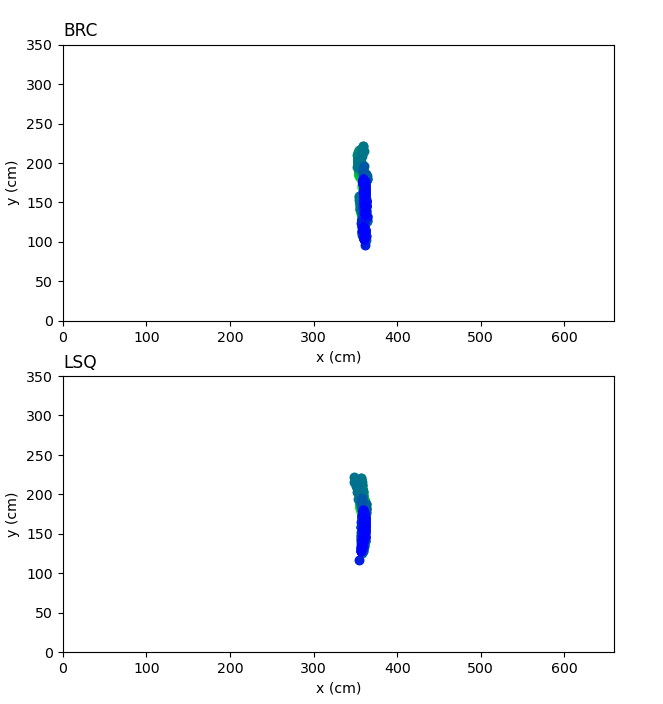
\includegraphics[width=8cm]{pictures/results_g3a.png}
\caption{Γραφική παράσταση για τα πείραμα \te{400\_170\_diag\_H\_B}}
\end{figure}
Όπως φαίνεται, φαίνεται η παρεμβολή του ανθρώπινου σώματος δημιουργεί έντονο θόρυβο, ο οποίος δεν είναι αμελητέος.

\subsubsection{\te{400\_170\_diag\_H\_C}}
Τέλος στο πείραμα \te{400\_170\_diag\_H\_C} ένας άνθρωπος κάλυπτε με τα χέρια του το \te{tag} απο όλες τις πλευρές για τα πρώτα τριάντα δευτερόλεπτα
του πειράματος και έπειτα σταματούσε.
Στο σχήμα 4.20 βλέπουμε τις χρονοσειρές γωνιών για το πειράματα ενώ στο 4.21 βλέπουμε την γραφική παράσταση του.
\begin{figure}[H]
\centering
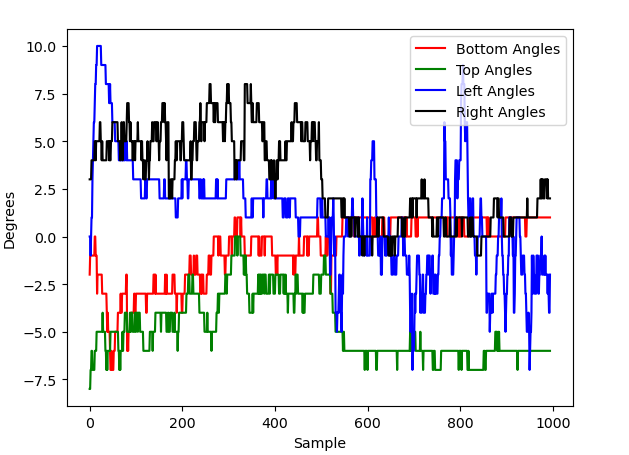
\includegraphics[width=8cm]{pictures/results_g4.png}
\caption{Χρονοσειρές γωνιών για τo πείραμα \te{400\_170\_diag\_H\_C}}
\end{figure}
\begin{figure}[H]
\centering
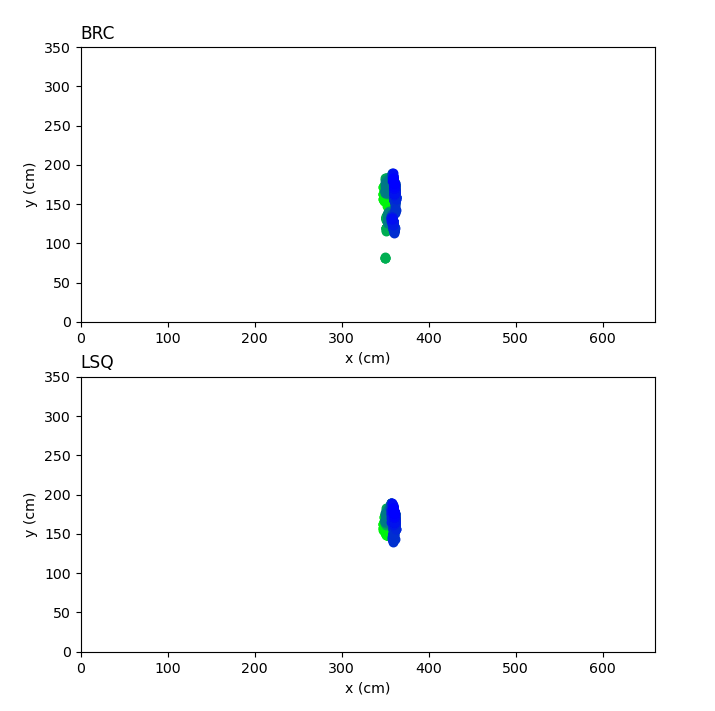
\includegraphics[width=8cm]{pictures/results_g4a.png}
\caption{Γραφική παράσταση για τo πείραμα \te{400\_170\_diag\_H\_C}}
\end{figure}
Φαίνεται πως ο θόρυβος των γωνιών μειώνεται περίπου στην μέση της χρονοσειράς.
Υπενθυμίζουμε πως τα σημεία χρωματίζονται απο πράσινα σε μπλέ με την σειρά που υπολογίζονται. Έτσι βλέπουμε πως τα πρώτα σημεία, δηλαδή αυτά που είναι πράσινα, είναι πιο διάσπαρτα, ενώ τα επόμενα, δηλαδή αυτά που είναι μπλέ, συγκλίνουν πιο καλά σε μια τοποθεσία.

\section{Πειράματα Κίνησης με Απρόσκοπτο \te{Line of Sight}}
Παρακάτω θα παρουσιάσουμε τα αποτελέσματα μας για τα πειράματα κίνησης στα οποία δεν υπήρχαν εμπόδια στο \te{Line of Sight}.
\subsubsection{Κίνηση Ευθείας Γραμμής}
Η πρώτη περίπτωση που θα παρουσιάσουμε είναι μια κίνηση σε ευθεία γραμμή κατα μήκος του δωματίου Α. Για αυτήν την κίνηση πραγματοποιήσαμε δυο πειράματα, στο πρώτο
το \te{tag} ξεκίνησε απο το αριστερό άκρο, \((157, 171)\), του δωματίου και κινήθηκε προς το δεξί άκρο , \((515, 175)\), ενώ στο δεύτερο πείραμα η κίνηση ήταν ανάποδη.
Στο σχήμα 4.22 φαίνεται η γραφική αποτύπωση των δυο περιπτώσεων.
\begin{figure}[H]
\centering
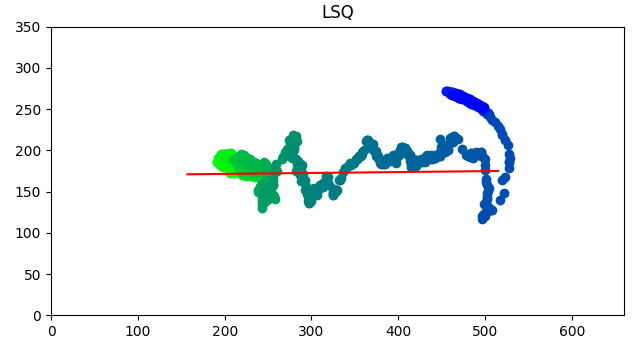
\includegraphics[width=7.5cm]{pictures/mov_lr.png}
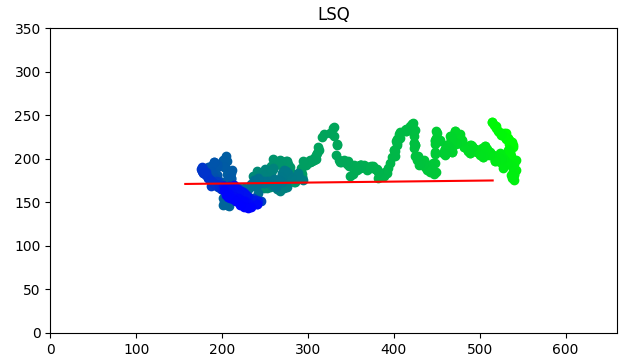
\includegraphics[width=7.5cm]{pictures/mov_rl.png}
\caption{Γραφική παράσταση για τα πειράματα ευθείας γραμμής, αριστερά προς δεξιά\te{(a)} και δεξιά προς αριστερά\te{(b)}}
\end{figure}

Για την περίπτωση αριστερά προς δεξιά το μέσο σφάλμα μεταξύ των σημείων και της ιδανικής ευθείας είναι 36 εκατοστά ενώ η τυπική απόκλιση είναι 32.4 εκατοστα.
Για την περίπτωση δεξιά προς αριστερά το μέσο σφάλμα είναι 19 εκατοστά ενώ η τυπική απόκλιση είναι 15.3 εκατοστα.

Επίσης έχει ενδιαφέρον να παρουσιάσουμε τις χρονοσειρές γωνιών τουλάχιστον για την περίπτωση αριστερά προς δεξιά, οι οποίες φαίνονται στο σχήμα 4.23

\begin{figure}[H]
\centering
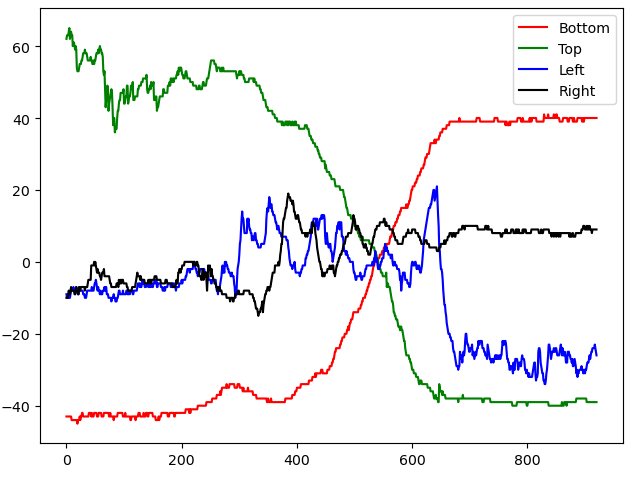
\includegraphics[width=8cm]{pictures/mov_lr_angles.png}
\caption{Χρονοσειρές γωνιών για την κίνηση αριστερά προς δεξιά}
\end{figure}

Το σχήμα 4.23 μας δίχνει γραφικά την μεταβολή των γωνιών \te{Top \& Bottom} απο την αριστερή προς την δεξιά θέση του δωματίου.


\subsubsection{Κίνηση Ορθογώνιου Παραλληλόγραμμου}
Παρακάτω παρρουσιάζουμε τα πειράματα για κίνηση η οποία διαγράφει ενα ορθογώνιο παραλληλόγραμμο, στο σχήμα 4.24 παρουσιάζονται οι γραφικές παραστάσεις για δύο επαναλήψεις του
πειράματος. Η πρώτη (4.24\te{a}) έγινε σε αργή κίνηση ενώ η δεύτερη (4.24\te{b}) έγινε σε γρήγορη κίνηση.
\begin{figure}[H]
\centering
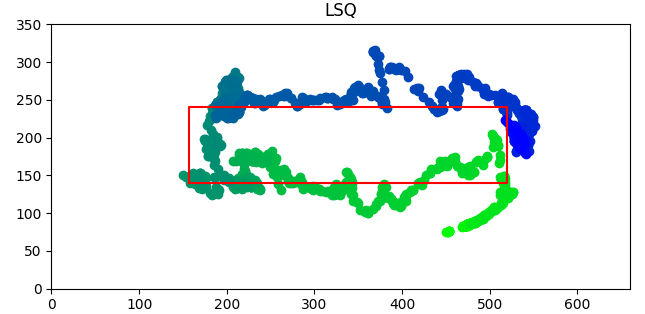
\includegraphics[width=7.5cm]{pictures/mov_sq1.png}
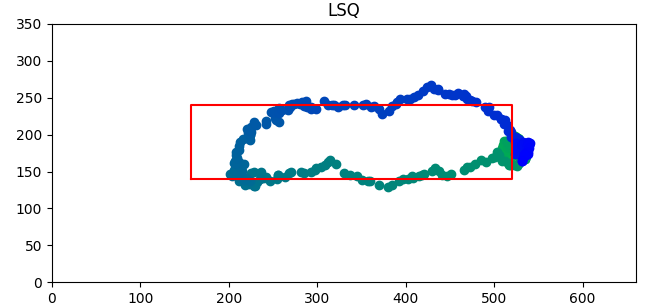
\includegraphics[width=7.5cm]{pictures/mov_sq2.png}
\caption{Γραφική παράσταση για την κίνηση ορθογώνιου παραλληλόγραμμου, αργή κίνηση\te{(a)} και γρήγορη κίνηση\te{(b)}}
\end{figure}

Αρχικά βλέπουμε πως στην περίπτωση της αργής κίνησης τα σφάλματα και η τυχαιότητα προλαβαίνουν να αλλοιώσουν τα αποτελέσματα περισσότερο απο την περίπτωση της γρήγορης κίνησης.
Στην αργή περίπτωση βλέπουμε πως το σφάλμα σε ορισμένες περιπτώσεις φτάνει εώς και 80 εκατοστά ενώ στην γρήγορη περίπτωση το μέγιστο σφάλμα είναι περίπου 70 εκατοστά αλλά
η γενική εικόνα είναι πολύ πιο ομαλή.

\subsubsection{Συνδιαστικές Κινήσεις}
Τέλος παρουσιάζουμε δυο πειράματα που διαγράφουν μια κίνηση τύπου Χ μέσα στο δωμάτιο και μια κίνηση με εναλλασόμενες μικρές αλλαγές κατεύθυνσης.
Στο σχήμα 4.25\te{a} και 4.25\te{b} φαίνονται τα δυο αυτά πειράματα αντίστοιχα.
\begin{figure}[H]
\centering
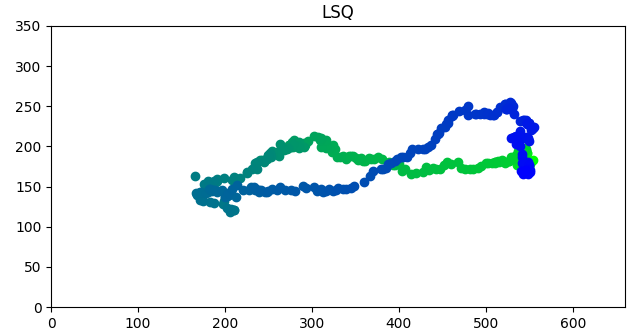
\includegraphics[width=7.5cm]{pictures/mov_x.png}
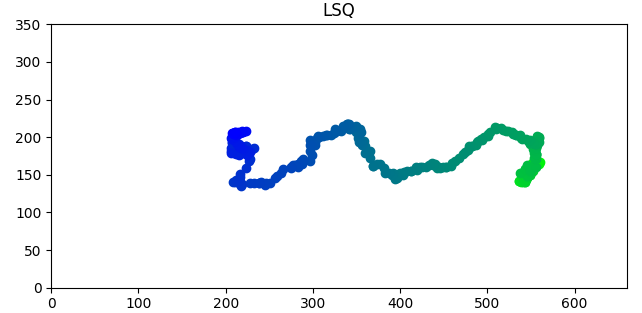
\includegraphics[width=7.5cm]{pictures/mov_zz.png}
\caption{Γραφική παράσταση για τις δυο συνδιαστικές κινήσεις}
\end{figure}

Φαίνεται πως λόγω της υψηλής λεπτομέρειας σε αυτές τις δυο κινήσεις, οι γραφικές παραστάσεις των πειραμάτων δεν είναι ιδιαίτερα ακριβείς.

\section{Πειράματα Κίνησης με Ανθρώπινο Εμπόδιο}
\subsubsection{Κίνηση Ευθείας Γραμμής}
Αρχικά επαναλάβαμε τα πειράματα ευθείας γραμμής με το ανθρώπινο σώμα να καλύπτει την μια μεριά του \te{tag}.
Στο σχήμα 4.26 φαίνεται η γραφική παράσταση και οι χρονοσειρές γωνιών για την περίπτωση κατα την οποία η κίνηση γίνεται αριστερά προς δεξιά και το ανθρώπινο σώμα
καλύπτει την αριστερή μεριά του \te{tag}.
\begin{figure}[H]
\centering
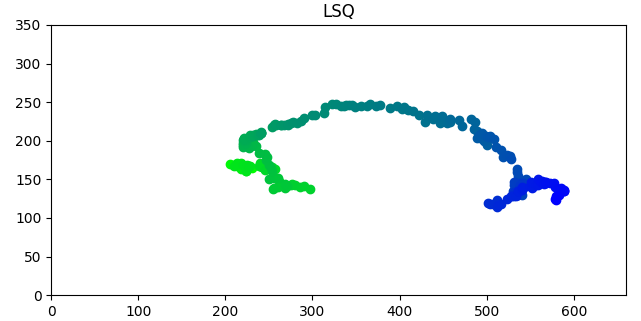
\includegraphics[width=10cm]{pictures/mov_H_lr.png}
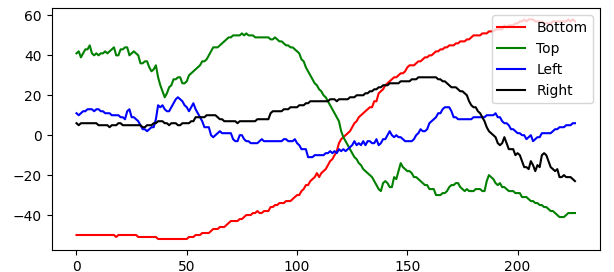
\includegraphics[width=10cm]{pictures/mov_H_lr_angles.png}
\caption{Γραφική Παράσταση\te{(a)} και Χρονοσειρές Γωνιών\te{(b)} για Κίνηση Αριστερά προς Δεξιά με Ανθρώπινο Εμπόδιο}
\end{figure}

Αρχικά βλέπουμε προφανώς πως τα αποτελέσματα είναι λιγότερο ακριβή. Έπειτα στις χρονοσειρές των γωνιών βλέπουμε να αντικατοπτρίζεται η μεταβολή των \te{Top \& Bottom} γωνιών
με αρκετά πιο έντονη συμβολή θορύβου. Μια ενδιαφέρουσα παρατήρηση είναι πως ενώ καλύπτεται η αριστερή μεριά του \te{tag} υπάρχει έντονος θόρυβος ακόμα και στο δεξί \te{anchor}.

Στο σχήμα 4.27 παρουσιάζουμε το ίδιο πείραμα με κίνηση απο δεξιά προς αριστερά και την δεξιά μεριά του \te{tag} να καλύπτεται.
\begin{figure}[H]
\centering
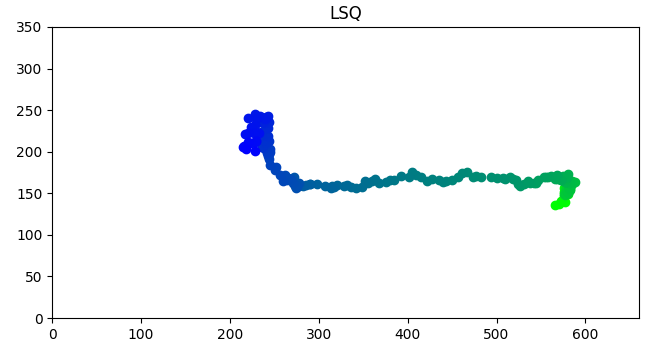
\includegraphics[width=10cm]{pictures/mov_H_rl.png}
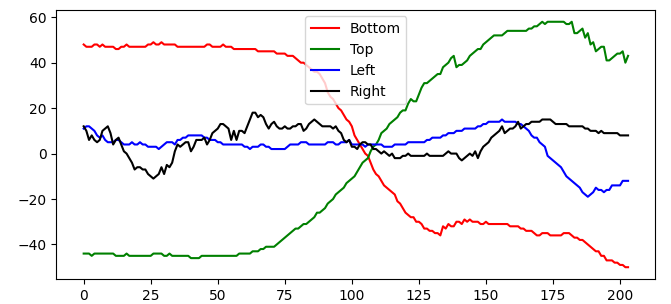
\includegraphics[width=10cm]{pictures/mov_H_rl_angles.png}
\caption{Γραφική Παράσταση\te{(a)} και Χρονοσειρές Γωνιών\te{(b)} για Κίνηση Δεξιά προς Αριστερά με Ανθρώπινο Εμπόδιο}
\end{figure}

Εδώ μπορούμε να δούμε με μια γραφική εποπτεία πως τα αποτελέσματα είναι καλύτερα απο την προηγούμενη περίπτωση, με την μεταβολή των γωνιών να φαίνεται πολύ καθαρά.
Μια ελαφρώς αντιφατική παρατήρηση είναι πως η γραφική παράσταση αυτής της κίνησης με ανθρώπινο εμπόδιο είναι καλύτερη απο τις παραστάσεις των κινήσεων χωρίς εμπόδιο.
Αυτό το αποδίδουμε στον θόρυβο του περιβάλλοντος που επηρέασε τις μετρήσεις μας για τα πειράματα χωρίς ανθρώπινο εμπόδιο.

\subsubsection{Κίνηση Ορθογώνιου Παραλληλόγραμμου}
Έπειτα επαναλαμβάνουμε το πείραμα για την κίνηση ορθογώνιου παραλληλόγραμμου. Στο σχήμα 4.28 βλέπουμε τις παραστάσεις για δυο επαναλήψεις αυτού του πειράματος.
\begin{figure}[H]
\centering
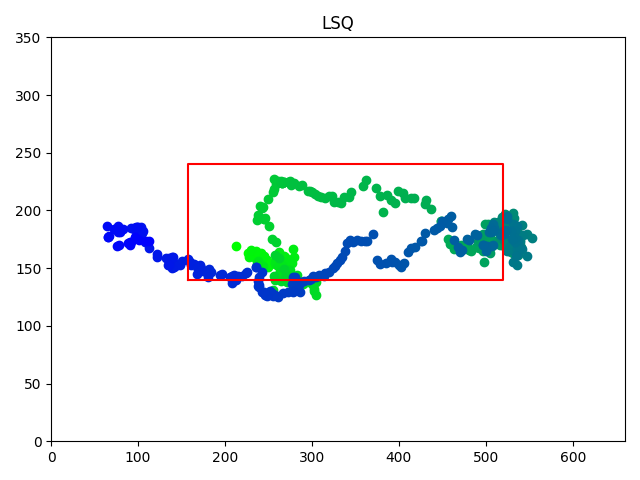
\includegraphics[width=7.5cm]{pictures/mov_sq_H_1.png}
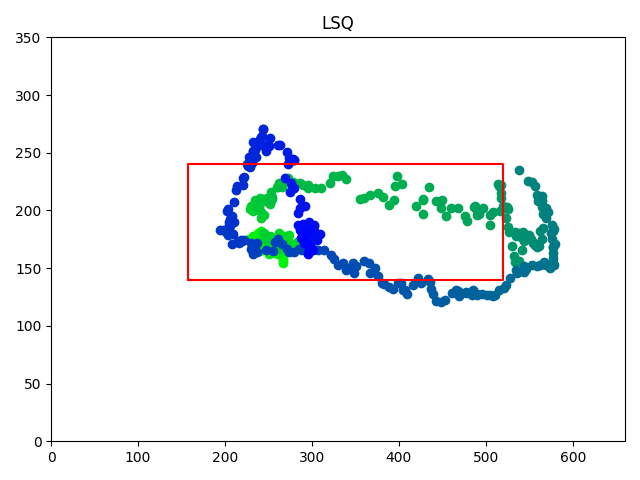
\includegraphics[width=7.5cm]{pictures/mov_sq_H_2.png}
\caption{Γραφικές Παραστάσεις για την Κίνηση Παραλληλόγραμμου με Ανθρώπινο Εμπόδιο}
\end{figure}

Όπως και στις προηγούμενες περιπτώσεις τα αποτελέσματα είναι αλλοιωμένα σε εμφανή βαθμό. Παρόλαυτά η γενική διαδρομή που ακολούθησε το \te{tag} είναι ακόμα εμφανής.

Εν τέλη είναι προφανές πως το ανθρώπινο σώμα σαν εμπόδιο μειώνει την ακρίβεια του συστήματος σε έντονο βαθμό.

\section{Φιλτράρισμα σε Πειράματα Κίνησης}
Σε αυτό το σημείο είναι η ώρα να εξετάσουμε μερικές μεθόδους για να βελτιώσουμε την ποιότητα των αποτελεσμάτων για τα πειράματα κίνησης. Θα μελετήσουμε
μερικά βασικά φιλτραρίσματα, συγκεκριμένα θα μελετήσουμε τι συμβαίνει οταν φιλτράρουμε τα δεδομένα των γωνιών, τι συμβαίνει οταν
φιλτράρουμε τα σημεία που παράγονται σαν αποτελέσματα και τέλος τι συμβαίνει οταν συνδιάζουμε τις δυο τεχικές μαζί.

Σε όλες τις περιπτώσεις θα βασιστούμε στην δεύτερη επανάληψη του πειράματος παραλληλόγραμης κίνησης με ανθρώπινο εμπόδιο, δηλαδή στο σχήμα 4.28\te{b}.
\subsection{Φιλτράρισμα Γωνιών}
Αρχικά πρέπει να δούμε τι συμβαίνει όταν φιλτράρουμε την αρχική μας πληροφορία. Για αυτό θα εφαρμόσουμε ένα φίλτρο \te{moving average} με διάφορα μεγέθη παράθυρου.
Στο σχήμα 4.29\te{a, b \& c} βλέπουμε τα αποτελέσματα για παράθυρο μισού, ενός και δυο δευτερολέπτων αντίστοιχα.
\begin{figure}[H]
\centering
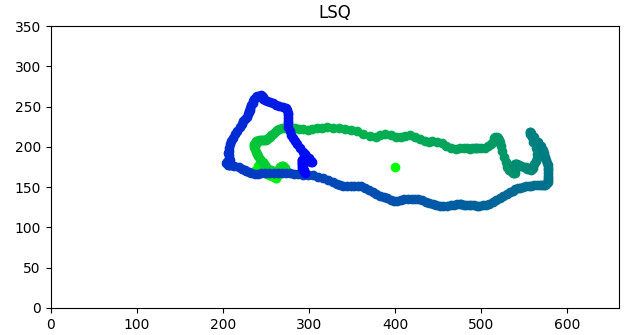
\includegraphics[width=7.5cm]{pictures/mov_sq_filt_05.png}
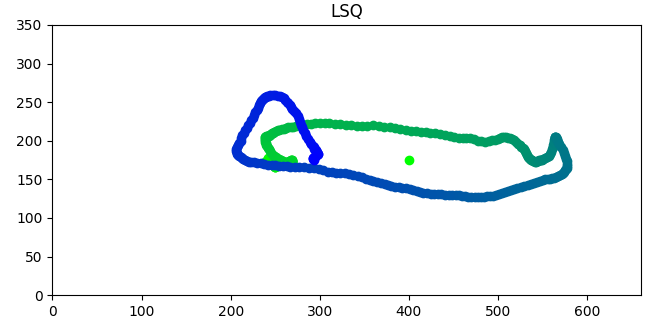
\includegraphics[width=7.5cm]{pictures/mov_sq_filt_1.png}
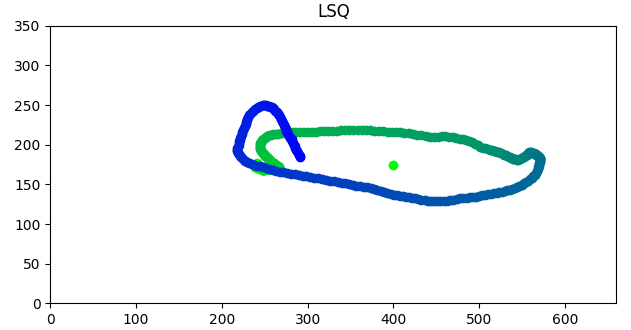
\includegraphics[width=7.5cm]{pictures/mov_sq_filt_2.png}
\caption{Κίνηση Παραλληλογράμμου με Φιλτράρισμα στις Γωνίες για Παράθυρο μισού, ενός και δυο Δευτερολέπτων}
\end{figure}

Αρχικά βλέπουμε πως σε σχέση με το σχήμα 4.28\te{b} τα αποτελέσματα είναι σαφώς καλύτερα σε κάθε περίπτωση.
Για παράθυρο μισού δευτερολέπου το \te{smoothing} δεν ειναι τόσο έντονο, ενώ για παράθυρο 2 δευερολέπτων χάνετε η διακριτική ικανότητα για γρήγορες κινήσεις. Για αυτό
καταλήγουμε στο παράθυρο ενός δευτερολέπτου.

\subsection{Φιλτράρισμα Σημείων}
Στην συνέχεια θα δούμε τι συμβαίνει αν φιλτράρουμε μόνο τα αποτελέσματα στην έξοδο του συστήματος. Στο σχήμα 4.30\te{a \& b} βλέπουμε αποτελέσματα για παράθυρο μισού και
ενός δευτερολέπτου.
\begin{figure}[H]
\centering
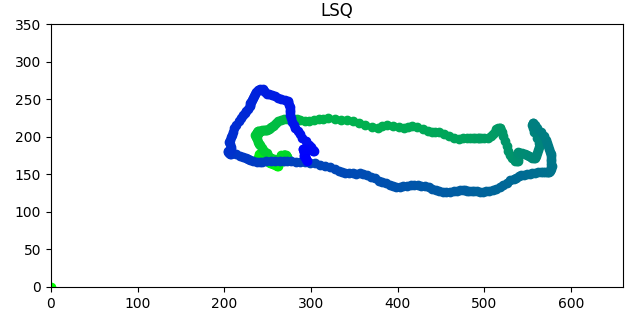
\includegraphics[width=7.5cm]{pictures/mov_sq_filt_p_05.png}
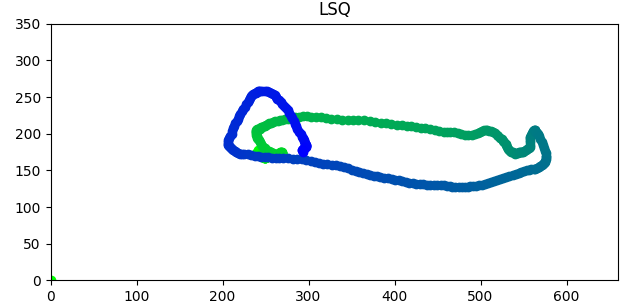
\includegraphics[width=7.5cm]{pictures/mov_sq_filt_p_1.png}
\caption{Κίνηση Παραλληλογράμμου με Φιλτράρισμα στα Αποτελέσματα για Παράθυρο μισού και ενός Δευτερολέπτου}
\end{figure}

Βλέπουμε πως τα αποτελέσματα είναι σχεδόν ίδια με την περίπτωση που φιλτράραμε τις γωνίες εισόδου.

\subsection{Φιλτράρισμα Γωνιών και Σημείων}
Τέλος στο σχήμα 4.31 βλέπουμε το αποτέλεσμα του πειράματος αν φιλτράρουμε τόσο τις γωνίες όσο και τα σημεία με ένα παράθυρο ενός δευτερολέπτου.
\begin{figure}[H]
\centering
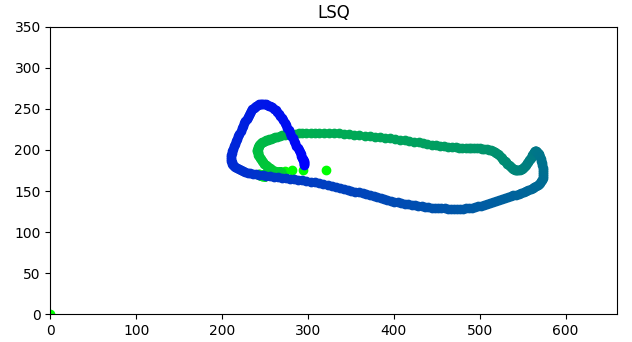
\includegraphics[width=7.5cm]{pictures/mov_sq_filt_ap_1.png}
\caption{Κίνηση Παραλληλογράμμου με Φιλτράρισμα στις Γωνίες και στα Αποτελέσματα για Παράθυρο ενός Δευτερολέπτου}
\end{figure}

Βλέπουμε πως η βελτίωση δεν είναι ιδιαίτερα μεγάλη καθώς το φιλτράρισμα \te{Moving Average} σταματάει να είναι αποδοτικό αν τα δεδομένα του είναι ήδη φιλτραρισμένα.
Παρολαυτά βλέπουμε πως το φιλτράρισμα είναι μια εύκολη και πολυ αποδοτική τεχνική για να εξομάλυνουμε τα αποτελέσματα μας.
